\chapter{Definitions and Related Work}
\label{chap:concepts}
In this chapter we repeat basic concepts related to the topic of this thesis by defining them and providing an overview about the current literature. The order of definitions is not alphabetical - instead content-related definitions are grouped together. Related work can be summarized to the following research areas: business information visualization,  time-oriented data visualization, large scale visualization and surveys of visualization tools. 

\section{Definitions}
\textbf{Information Visualization} is the graphical representation of non-spatial or abstract data  \cite{Keim2006}. In contrast to scientific visualization, data information visualization does not have an inherent 2D or 3D structure  \cite{Shneiderman2008} and thus, no spatial relation. Abstract data usually exists in data tables with rows and columns. These columns are mapped in Information Visualization to graphical attributes such as position, color, size, orientation, texture or hue. 
Since business data is usually abstract, discrete and multivariate  \cite{Tegarden1999}, the type of visualization for business data is Information Visualization.
\par
\textbf{Data visualization} is a more general term for generating a graphical representation with data and is used in Business Intelligence (\gls{BI}), Analytics, data discovery and in visual analytics.
\par
\textbf{Business Information Visualization} (\gls{BIV}) \label{BIV} is defined as the use of visualization technologies to visualize business data  \cite{Tegarden1999}. While business data appears in multiple applications, \gls{BIV} is usually achieved with the help of computer tools - ranging from data loading to interactive visual analysis. Interactive visual analysis in businesses is often used to do self-service data science \cite{Russom2011,Parenteau2016,SAS2012,Curran2005}. \textbf{Self-Service} data visualization describes an approach that encourages a broad public to do data analysis with easy-to-use tools.
\par
\textbf{Advanced Data Visualization} (\gls{ADV}) in our understanding is a visualization technique which is able to scale to large and huge amounts of data.
\par
\textbf{Large Data}: To characterize the data volume we follow a definition of Huber. He divided data into small, medium, large, huge and massive data. Large data according to  \cite{Huber1994} is defined as data sets with $10^6$ and huge data with $10^8$ data entries. We are considering large and huge amounts of data.
\par
\textbf{Abstract data} is defined as data without any spatial relationship in the data  \cite{Shneiderman1996}. 
\par
\textbf{Discrete data} is data which can be mapped to integer values.
\par
\textbf{Multivariate data} is often mixed-up with the term multi-dimensional. For this reason we define  multivariate data by the number of dependent attributes. If the data set holds more than two dependent attributes then we call the data \textit{multivariate}. In contrast, multi-dimensional depicts the number of independent attributes of a data set \cite{Aigner2011}.
Multivariate time series are time series where one data item holds several variables at the same point of time \cite{Aigner2011}. In the analysis of multivariate time series of different variables and their combinations are interesting. In order to gain understanding of their development over time, the challenge of multivariate data is the selection of meaningful dimensions and their visualizations. 
\par
\textbf{Visual Scalability}\label{scalability} or "perceptual scalability" is defined as the capability of visualization tools to display large data sets in an effective manner  \cite{Eick2002}\label{effective}. In the context of time-oriented business data \textbf{effective} means the presentation of patterns to support the user tasks. To measure the visual scalability of different visualization techniques for time-oriented data we refer to the work of Eick  \cite{Eick2002}. He proposed to measure visual scalability by the database metrics of the data set and the visual characteristics of the visualization technique.
\par
\textbf{Database metrics}\label{databasemetrics} assess the size of the database in bytes, in rows or in columns \cite{Eick2002}. For multi-dimensional data, database metrics are a combination of the number of rows and columns.
\par
\textbf{Visualization characteristics} describe the number of elements and attributes presented on the screen and measure how many distinct items a visualization technique can display \cite{Eick2002}. This number is measured at the visualization technique level.
\par
\textbf{Visualization Tools}\label{tools} are computer tools and frameworks which offer a range of chart types to support visual data exploration. Tools for visual data exploration have different purposes which range from Business Intelligence (\gls{BI}) and Analytics, data discovery, data mining to visualization tools. Since the differentiation between those tools is not selective and the terms are not clearly distinguished we make the following differentiation:
Data mining tools cover the extraction of patterns and model the underlying data structure  \cite{FerreiradeOliveira2003}. Data mining is based on automated algorithms which detect relevant patterns and display the results in terms of statistical reports or visualizations. In contrast to automated analysis, \textbf{visual data exploration} (\gls{VDA}) is a human guided process  \cite{FerreiradeOliveira2003}. First, data is displayed on the screen as a visualization and with the help of human visual capabilities new hypotheses are formed. With visualization tools the user can interact with the data by changing parameters, filtering, zooming and defining new user input. Visualization tools can denote both tools to represent data mining results and tools for \gls{VDA}. We will use visualization tool in terms of a tool which supports visual data exploration. 


% \iffalse
% Data Mining tools allow automatic decision-making by algorithms which are applied to the data and extract patterns in an automatic way  \cite{Goebel1999}. Exploratory data analysis (EDA) tools are used to mine data with support of human input. We will use the definition of EDA tools for  visualization tools in this work. As a pwc-survey showed eventhough automatic ways for decision support exist data analysis still relies on human judgement and thus  \cite{PwC2016}, visualization tools are used to support the business user in the data discovery process. The main goal of visualization tools is the user support in gaining insights into the data. 
% Visualization tools display hundreds of items on the screen and offer interaction techniques such as zooming and filtering  \cite{Shneiderman2008}.
% \fi

\textbf{Visualization techniques} denote the way in which data variables are mapped to graphical primitives. To avoid the redundant use of the term visualization we will call visualization techniques simply \textit{techniques} in the following work. Typical examples for techniques are bar charts, line charts or scatter plots. 
\par
\textbf{Visual Metaphor: } Every technique has its own characteristic in presenting data. These characteristics include visualization attributes, the mapping, the use of aggregation methods and dimensionality. Visualization characteristics are called the visual metaphor of a technique  \cite{Tegarden1999}. Each metaphor has its own strengths and weaknesses with respect to scalability and its particular application. 

\par
\textbf{Time-oriented Data}: Data which is linked to time\cite{Aigner2011} is called \textit{time-oriented data}. Time-oriented data has specific characteristics such as being linear/cyclic, discrete/continuous or event-based/interval-based. Data that shows seasonal behavior is called cyclic while data without that characteristic is linear. Discrete time can be mapped to integer values and continuous time to real numbers. Events have no duration while time spans are intervals. In the following work, we will use time-oriented data and large data equivalently for large time-oriented data.
\par
\textbf{Time Series}: Univariate time-oriented data is called time series \cite{Aigner2011,  Buono2005,  Walker2016,  Leonard2005,  Chen1993,  Esling2012}.
\par

\iffalse
Decision-makers usually are part of a company's management and thus the majority of them use these tools with limited programming knowledge. Therefore, tools have to be self-explaining, easy-to-use  \cite{Crapo2000} and without the requirement of extensive programming\label{user}. Visualization plays an important role as it reduces information overload  \cite{Keima} and simplifies the process of problem-solving  \cite{Zhang}. Even though we only consider visualization tools which are used to explore data, visualization tools have two roles: presentation and exploration  \cite{Crapo2000}. Visualization as presentation is either used to display data without any data mining algorithm or it is used to present the results of a data mining algorithm. Visualization as exploration is used before and during the data mining algorithm to explore the data interactively. This group is called visual analytics. The decision-maker needs both processes for decision making as results are presented on the screen and to explore the data interactively  \cite{Ware2012}. 
An important data type for business is time-oriented data(\ref{data}) as it allows businesses for analyzing the past and predict the future of the company  \cite{Ao2010}. We will have a closer look at user tasks in section \ref{tasks}.
\fi


\section{Related Work}\label{chap:related}
%: Topic Business Information Visualization
\subsection{Business Information Visualization}
Although Information Visualization is intensively researched  \cite{Shneiderman2008,  Shneiderman2002,  Shneiderman1996,  Keim2002, yi2008understanding, Liu2014, Lee2016, Ellis2007, Ware2012, Kreuseler2000} only few researchers have written specifically about \gls{BIV} \cite{Bacic2012, Bacic2013, Zhang1995, Zhang1998, Zhang2001}. Card et al. described how Information Visualization amplifies cognition \cite{Card1999}. Since visualization acts as an increased resource to store information beyond the brain's capacity, visualization also supports the business-related process of problem solving  \cite{Bacic2012}. This psychological view of the business user is explored by Bačić \cite{Bacic2013,  Bacic2012}. He studied the process of knowledge creation in Business Intelligence. Bačić et al. outlined that \gls{BIV} reduces information complexity and information uncertainty and thus, supports the business user in decision-making \cite{Bacic2012, Bacic2013}. In order to reduce complexity Bačić et al. suggest to reduce visual clutter.
 A more generalized perspective is covered by Tegarden. He defined \gls{BIV} and considered data types and appropriate visualizations that are used in \gls{BIV}. Zhang  \cite{Zhang1995,  Zhang1998,  Zhang2001} described the scope of \gls{BIV}. According to her, \gls{BIV} has to deal with non-geometric data and on the other side consider the human problem-solving process \cite{Zhang2001}.  The related works to \gls{BIV} are the foundation for this work's definition of user tasks. 
 
\par
\pagebreak
% Topic: Time-oriented Data visualization
\subsection{Time-oriented data}
Leonard emphasized the role of time-oriented data in business. Time-stamped data can help managers to make better decisions \cite{Leonard2005}. 
%Time-oriented data appears in the literature as  time-dependent  \cite{Mueller2003,  Tominski2005,  Kriglstein2014,  Aigner2007,  VanBuuren2001,  FerreiradeOliveira2003,  Yang2003,  Chung2014,  Rind2011},  time-varying  \cite{Moere2004},  time-oriented  \cite{Aigner2008,  Aigner2007,  Aigner2011,  Hinum2005,  Walker2016} or time-related  data \cite{Keim2004}. 
Significant work on the visualization of time-oriented data was done by Aigner \cite{Aigner2011,  Aigner2008,  Aigner2007} who proposed a taxonomy for the time-domain and various visualization techniques. He summarized the key criteria of time-oriented data which influence visualization, the \textit{frame of reference} and the \textit{number of variables}. The frame of reference differentiates between abstract and spatial. The number of variables divides data into univariate and multivariate. 
Other differentiations concerning time were published by Kriglstein et al \cite{Kriglstein2014}. Their hypothesis is that time-oriented data can be presented in two ways: either by \textit{animation} or by using \textit{space-metaphors}. One example for a space-metaphor is a time-line where time is mapped to a line. In their work they collected experimental findings for animation and space-metaphors. These studies compared animation,  small multiples and traces. The result was that none of them is able to scale beyond 200 data items  \cite{Robertson2013}. Instead they suggested to use temporal abstraction for analyzing large time-oriented data sets which is explained in detail in section \ref{temporalabstraction}.  Aigner et al.'s survey of visualization techniques for time-oriented data provides the basis of our selection of studied visualization techniques \cite{Aigner2011}. Some of the analyzed visualization techniques in this work were developed to analyze business data such as Spiral Graphs \cite{Weber2001} or Recursive Patterns \cite{Keim1995}. 
\par
% Topic: Large scale data visualization
\subsection{Large scale data visualization}
Time-oriented data is often described as data with high volume - large data \cite{Leonard2005, Lin2005}. The problem of large scale data visualization is known in literature as
\textit{large}  \cite{PiringerHarald2011,  Keim2001,  Keim1996,  Tennekes2013,  Yang2003,  Keim2005,  Wickham2013}, \textit{large-scale}  \cite{Leonard2005,  PiringerHarald2011,  Cuzzocrea2011,  Keim2005},  \textit{Big Data} \cite{Patil,  Keahey2013,  Chen2012} and \textit{data-intensive}  \cite{PhilipChen2014,  S.MD.Mujeeb2005}. One challenge of large scale data visualization is the perceptual scalability \cite{Wang2015}. Visualizations must provide an overview to the user \cite{Shneiderman2008}. One interpretation of providing that overview is to plot the complete data set. However, when plotting the whole data set overplotting occurs. If data is reduced, data reduction can destroy patterns in the data. In order to solve visual clutter there exist three approaches: scalable visualization techniques, data reduction and interaction \cite{Krzywinski2009,  Luo2012,  Fekete2002}.  A collection of  clutter reduction techniques can be found in \cite{Ellis2007}.
\par
\textbf{Data reduction techniques} are known in the literature as \textit{data aggregation and dimension reduction} \cite{FerreiradeOliveira2003,Aigner2011, Keim2005}. Data reduction reduces data rows while dimension reduction condenses columns. Examples for data reduction are sampling and filtering \cite{Fisher2012, Fekete2002}, hierarchical aggregation \cite{Elmqvist2010}
%as a method to reduce visual clutter in visualizations  which builds aggregated data items by forming a tree structure and collapsing the children of a tree. Liu et. al. studied 
, binned and pixel-aware aggregation \cite{Liu2013, Li2016}. 
%Binned aggregation divides data into adjacent bins and combines them for aggregation. Pixel-aware aggregation clusters pixels according to their screen coordinates. 
Jugel et al. dealt with the aggregation of time-series aggregation \cite{Jugel2014}. The M4 aggregation compresses time series data into a set of equidistant time spans. \\
\textbf{Dimensionality reduction} techniques are Principal Component Analysis (\gls{PCA})  \cite{Aigner2008}, K-Means Clustering  \cite{Hamilton2015}, Multi-Dimensional Scaling or  Self-Organizing Maps (\gls{SOM}) \cite{PiringerHarald2011}.
\par
\textbf{Scalable visualizations} are visualization techniques which can display large to huge data sets effectively following the definition of visual scalability by Eick \cite{Eick2002}. Eick described the \textit{number of insights} caused by a visualization tool\cite{Eick2002} as an ideal measure. The definition of insights differ from 'Aha' moments to knowledge building \cite{Batyrshin2007}. While 'Aha' moments can be measured by neural activity, knowledge building is harder to grasp. Since information visualization uses the term "insights" in both ways, Eick proposed to measure visual scalability in terms of database metrics and visual scalability.  We will stick to the definition of Eick.  
\label{related:class}
A taxonomy for scalable visualizations was proposed by Keim  in his taxonomy of visualization techniques \cite{Keim1996}. 
He  proposed five categories for visualization techniques for large data sets\cite{Keim1996}. \\*
\textit{Graph-based} techniques present large graphs by using layout algorithms  \cite{Keim1996, Noirhomme-Fraiture2002}.\\*
\textit{Geometric projection} techniques (GP-techniques) map multi-dimensional data to a 2D screen  \cite{FerreiradeOliveira2003}. A well-known example is the use of parallel coordinates \cite{Inselberg1990}, which maps $k$ attributes to $k$ parallel axes in the 2D plane. \\*
\textit{Pixel-oriented} techniques map each data item to one pixel on the screen. Position and color are used to represent data attributes  \cite{Keim1996, Keim1995,  Stein2013,  Keim2000,  Keim1996pixel,  Keim2001,  Keim2005,  Keim2008}.\\*
\textit{Hierarchical} techniques divide the k-dimensional space into subspaces and shows it hierarchically \cite{Yang2003, Shneiderman1992, LeBlanc1990}. An example technique would be TreeMaps \cite{shneiderman2001ordered}.\\*
\textit{Icon-based} techniques map each data item onto one icon. The attributes are mapped to different icon features  \cite{Keim2001, Chung2014,  Borgo2013,  Fanea2005}. Chernoff-faces and stick-figures belong to this class \cite{Keim2002}. \\
Besides scalable visualization techniques aggregated pixels became popular to present huge data. In order to emphasize the importance of aggregation Shneiderman proposes to adapt his visualization mantra to Big Data Visualization by aggregation markers \cite{Shneiderman2008}. The visualization mantra can be reinterpreted as "Overview first with the help of aggregation markers, zoom in and filter, then details on demand".
\par
\textbf{Interaction techniques }are one way to implement Shneiderman's mantra in visualization tools \cite{Paterno1997, Shneiderman1996}. Zooming and Filtering can present more details of the data \cite{Keim2000Tut}. Dynamic queries provide a filter-mechanism via multiple widgets, such as sliders or input fields  \cite{Hochheiser2004,Shneiderman2008,Aigner2011}. \\
\textbf{Distortion techniques} such as Perspective Walls are a known method for time-oriented data to provide Focus+Context \cite{Stroe1999, Aigner2011} and to facilitate navigation of large data set . Distortion techniques become an interaction technique when connected to the mouse cursor.  
The main idea of distortion techniques is to present relevant data enlarged in the user focus while less relevant data are shown in the periphery in a smaller presentation. \textit{Fish-eye} for example behaves similarly to a magnifying glass. Distortion techniques are not providing additional pixels to the existing screen pixels but enhance the screen space metaphor by prioritizing screen pixels. 
Examples for distortion techniques are \textit{Bifocal Displays}  \cite{Spence1982}, \textit{Fish-eye Views} and \textit{Perspective walls \cite{Keim2005},  \cite{Mackinlay1991}}.\\*
All distortion techniques transform the undistorted 2D space by a mathematical function and bring more relevant data points into focus.\\* 
\textit{Bifocal Displays} (figure \ref{fig:bifocal}) bend the space with a linear function.
\begin{figure}[H]
    \centering
        \scalebox{.25}{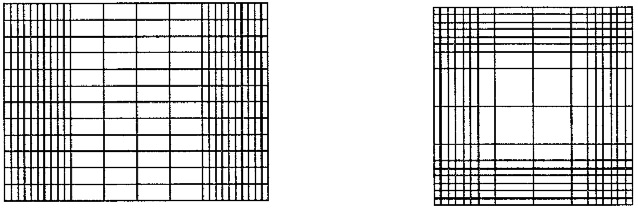
\includegraphics{src/images/f06b}}
    \caption[Bifocal Displays]{Bifocal Displays: distortion by linear function. From  \cite{Stroe1999}.}
    \label{fig:bifocal}
\end{figure}
\textit{Fish-eye Views} (figure \ref{fig:fisheye}) (also known as Table and Magnification Lense) apply a power function.
\begin{figure}[H]
    \centering
        \scalebox{.25}{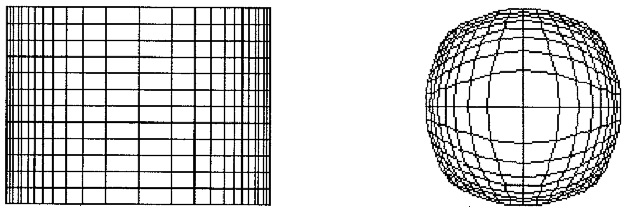
\includegraphics{src/images/f11c}}
    \caption[Fish-eye]{Fish-eye views:  distortion by a power function with an odd exponent  \cite{Stroe1999}.}
    \label{fig:fisheye}
\end{figure}

\textit{Perspective walls} (figure \ref{fig:perspectivewall}) distort the space by applying both linear and power function. Thus, a 3D-representation consisting of three walls is created. The front wall shows details and the two side walls provide context. 
\begin{figure}[H]
    \centering
        \scalebox{.25}{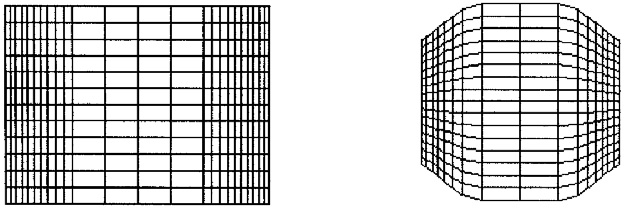
\includegraphics{src/images/f10b}}
    \caption[Perspective Walls]{Perspective Walls: distortion by a half linear and half power function. From  \cite{Stroe1999}.}
    \label{fig:perspectivewall}
\end{figure} 
\par
\textbf{Navigation techniques }include Brushing \& Linking \cite{Tegarden1999, Aigner2011}, Navigational Maps \cite{Keim2005} and Search \cite{Buono2005}. \\
\textit{Brushing \& Linking: }The user can select data items on the screen (Brushing) and the respective items are highlighted in every connected window (Linking) which is also known as coordinated window. Therefore, lasso, rubber-band or rectangular selection enables the user to select groups of data items. 
\par
Time-related interaction techniques are covered in \cite{Buono2005}. Buono et al. describe the system \textit{TimeSearcher} and the implemented interaction techniques for time-oriented data such as time-boxes. One interaction technique is pattern search. The user can draw a rectangular search box. The defined pattern is then searched in the data. Pattern search is one implementation of search as a navigation technique.\\
\par
In summary, all methods for clutter reduction in visualization tools support the business user in reducing information complexity. The proposed techniques can be divided into data reduction, visualization and interaction methods which is why this thesis applies this structure.
\par
\subsection{Big Data \& visualization tools}
% Topic: Survey of visualization tools
In chapter \ref{chap:Tools} we are comparing different \textbf{visualization tools}  and their ability to display large data. Wang et al. conclude that Big Data visualization tools perform poorly\cite{Wang2015}. In recently years many tools have been developed that promote themselves as able to handle Big Data \cite{Zoomdata2017, Datameer2017, Zeppelin2017}. Bikakis et al. surveyed different generic visualization systems and graph-based systems in the semantic web of Big Data \cite{Bikakis2016}. They compared the spectrum of analytical methods and visualization techniques. However, these systems are usually not used in business. 
Other tool comparisons are published by Zhang et al.  \cite{Zhang2012} and Patil  \cite{Patil}. These works compared commercial visual analytics system in the era of Big Data. Their key finding regarding visualization was the lack of support for advanced visualizations \gls{ADV}. In contrast Harger et al. surveyed open source visual analytics systems  \cite{Harger2012}. For \gls{BI} and Analytics the technology research center Gartner annually publishes a market overview of the most important \gls{BI} and Analytics tools which also serve for data discovery. The leading tools also appear in the survey  \cite{Evelson2012} regarding commercial advanced visualization tools and the works of Zhang  \cite{Zhang2012}. 
\par
In our work we survey time-oriented visualization techniques with regard to their scalability, makig use of existing taxonomies and scalability techniques. Our selection of tools were partially analyzed in other publications. However, the set of assessed criteria differed from ours.






